%%%%%%%%%%%%%%%%%%%%%%%%%%%%%%%%%%%%%%%%%%%%%%%%%%%%%
%			ŠABLONA PÍSNIČEK v. 18.09               %
%%%%%%%%%%%%%%%%%%%%%%%%%%%%%%%%%%%%%%%%%%%%%%%%%%%%%
% Tento soubor slouží jako (naučná) šablona, pomocí 
% které lze vytvářet zdrojové soubory k jednotlivým 
% písním.
%%%%%%%%%%%%%%%%%%%%%%%%%%%%%%%%%%%%%%%%%%%%%%%%%%%%%
%			Jak psát soubory songů?                 %
%%%%%%%%%%%%%%%%%%%%%%%%%%%%%%%%%%%%%%%%%%%%%%%%%%%%%
%	1. Text písně se začíná psát na místě START 
%	   a končí na místě END. Zbylý text ignorujte.
%	2. Jak bude vypadat pdf písně zjistíte po tom, 
%	   co soubor zkompilujete pomocí souboru   
%      ../Generator/generator. 
%	3. Při psaní dodržujte následující TeX pravidla:
%	 a) Nový řádek napíšete pomocí dvou odsazení 
%	    tedy dvou enterů.
%	 b) Nová sloka se píší pomocí \sloka a odsazení.
%		Refrén se píše jako \refren, v případě více 
%		refrénů \refren[č. refrénu].
%	 c) Akordy se píšou tak, že napíšete před slovo,
%	    kde chcete mít akord (bez mezery):
%		^{AKORD1\,AKORD2...}.
%	4. Pokud chcete ušetřit tvůrcům práci, tak 
%	   si přečtěte další poučný soubor o typografii 
%	   ../../Typo_pravidla.txt.
%	5. Akordy stačí psát jen do první sloky, když 
%	   se nezmění -- kytaristé to zvládnou
%	7. Název písně pište na místo [NÁZEV] a autora 
%	   pište na místo [AUTOR] 
%	7. Jak psát věci na české klávesnici:
%	   \ = alt gr + q; [/] = alt gr f/g; 
%      {/} = alt gr + b/n; ^ = alt gr + 3 , cokoliv
%%%%%%%%%%%%%%%%%%%%%%%%%%%%%%%%%%%%%%%%%%%%%%%%%%%%%
%			Jak kompilovat jednotlivé písně?        %
%%%%%%%%%%%%%%%%%%%%%%%%%%%%%%%%%%%%%%%%%%%%%%%%%%%%%
%	1. Více návodu je k tomuto napsáno v souboru 
%      ../Generator/generator. 
%%%%%%%%%%%%%%%%%%%%%%%%%%%%%%%%%%%%%%%%%%%%%%%%%%%%%
%			Jak kompilovat celý zpěvník?			%
%%%%%%%%%%%%%%%%%%%%%%%%%%%%%%%%%%%%%%%%%%%%%%%%%%%%%
%	1. Více návodu je k tomuto napsáno v souboru
%	   ../Cely_zpevnik/zpevnik.tex.
%%%%%%%%%%%%%%%%%%%%%%%%%%%%%%%%%%%%%%%%%%%%%%%%%%%%%
\begin{song}{title=\predtitle \centering Let Her Go \\\large Passenger }  %% sem se napíše jméno songu a autor

\vspace*{.5cm}

\begin{centerjustified}
\vetsi
{\centering 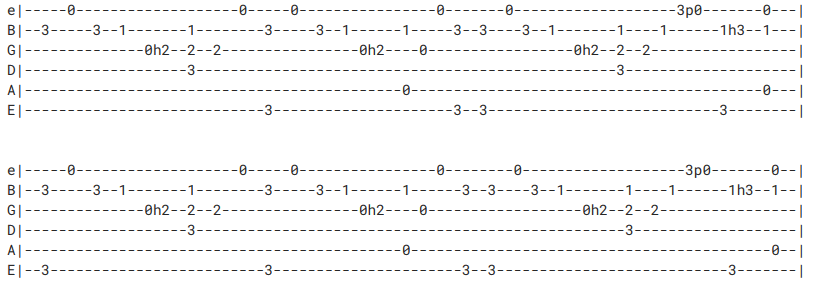
\includegraphics[scale=2.5]{../taby/LetHerGo.png}}

\refren
Well you only need the ^*{C}lig ht when its burning ^{\z G}low

Only miss the ^{D}sun when its starts to ^{\z Emi}snow

Only know you ^{C}love her when you let her ^{G}go

Only know you’ve been ^{C}high when youre feeling ^{\z G}low

Only hate the ^*{D}roa d when youre missin' ^{\z Emi}home~~

Only know you ^{C}love her when you've let her ^{G}go  ^{Dsus4}

And you let her go.

\textbf{Em   C   D   Bm   Em   C   Dsus4}

\sloka
^{Emi~z}Staring at the bottom of your ^{C}glass

Hoping ^{D\z}one day you will make a dream ^{Hmi\z}last.

The dreams come ^{Emi}slow and they go ^{C}so fast  ^{Dsus4}

You see her when you close your eyes

Maybe one day you will understand why

Everything you touch surely dies.


\end{centerjustified}
\newpage
\begin{centerjustified}
\refren
But you only need the light when it's burning low

Only miss the sun when it starts to snow

Only know you love her when you've let her go

Only know you've been high when you're feeling low

Only hate the road when you're missin home

Only know you love her when you've let her go.


\refren
Staring at the ceiling in the dark

Same ol' empty feeling in your heart.

Love comes slow and it goes so fast

Well you see her when you fall asleep

But to never to touch and never to keep

Because you loved her too much

And you dive too deep.


\refren
   And you let her ^{Emi\z}go~~~~

   Ooooo ^*{C}ooo oo ^{D}oooooo.

   And you let her go

   Ooooooo ooooo ooooo.

   And you let her go.

\textbf{C   D   Em   C   D}

\refren
   Cause you only need the ^*{\z C}lig ht when its burning ^{\z G}low~~

   Only miss the ^{D}sun when it starts to ^{\z Emi}snow~~

   Only know you ^*{\z C}lov e her when you've let her ^{\z G}go.~~  ^{D}

\end{centerjustified}
\setcounter{Slokočet}{0}
\end{song}
